This section provides an overview of \mfix's Discrete Element Modelling (DEM)
abilities. \mfix's DEM simulations retain all the functionality of MFIX-DEM. 
\mfix\ can be run in both a pure granular (particles only) mode  
as well as a particle fluid-coupling mode. In the latter case, \mfix\ models 
the fluid phase as a continuum and models the
particles of the solid phase individually. This approach supports a wide range 
of customization for particle dynamics, including mutliple particle collision 
force and drag schemes. For more information on the DEM capabilities of \mfix\
see \demdoc\ on the MFIX Documentation webpage at  
{\url{https://mfix.netl.doe.gov/download/mfix/mfix_current_documentation/dem_doc_2012-1.pdf/}}.  

\section{Overview}

\begin{figure}
    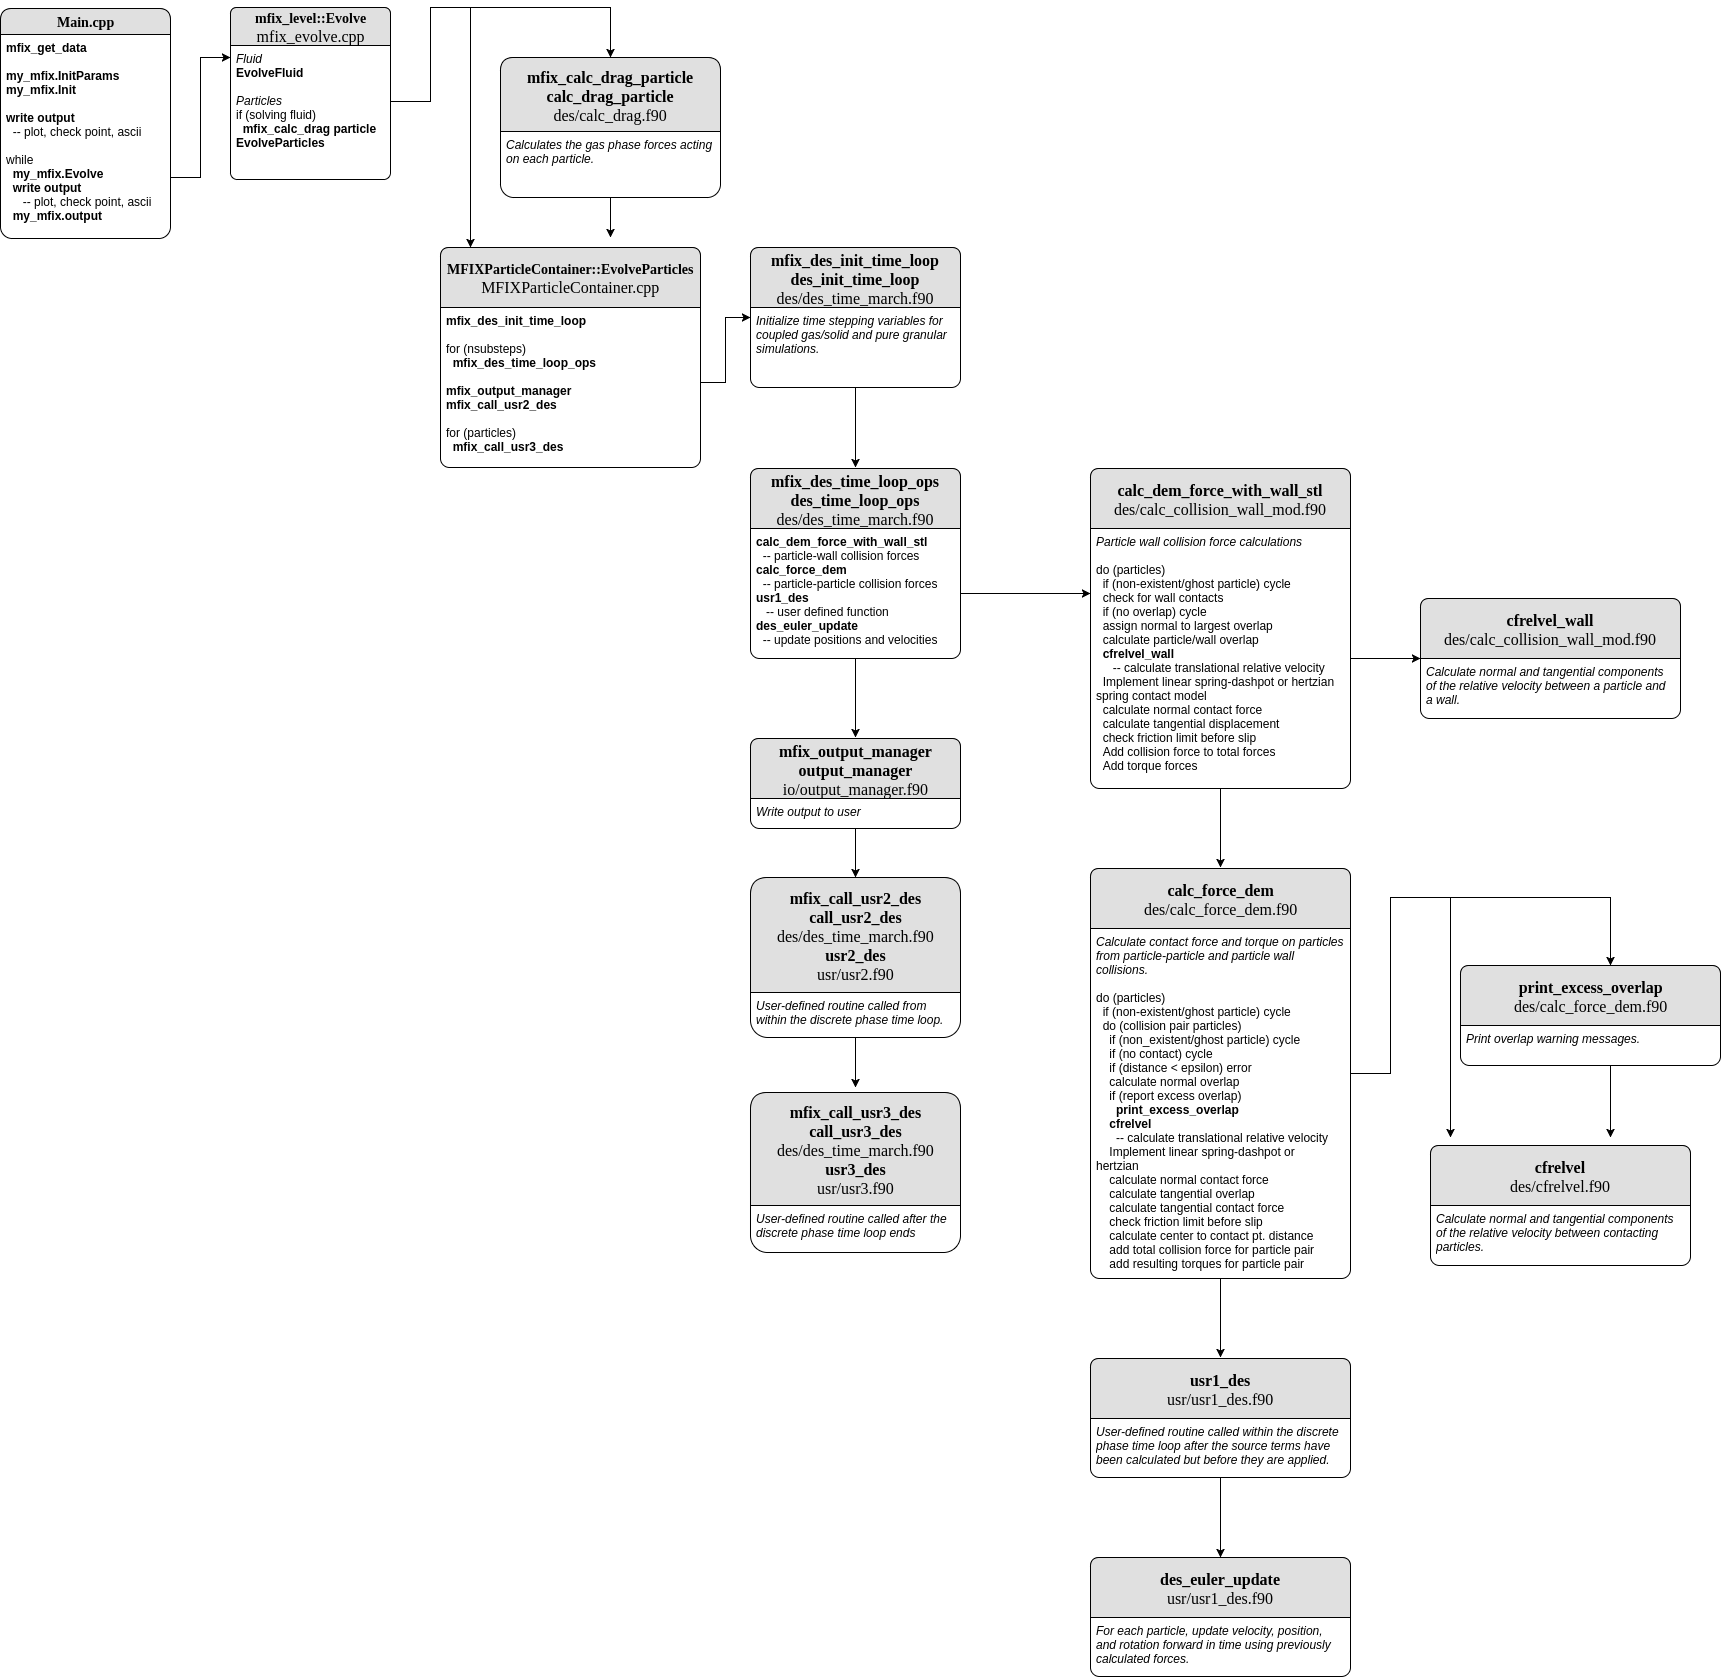
\includegraphics[width=\linewidth,natwidth=800, natheight=600]{./Particles/MFIX-Particle-Diagram.png} 
    \caption{Particle Routines Flowchart}
    \label{fig:pflowchart}
\end{figure}

\mfix\ retains all the functionality of MFIX-DEM. A detailed discription of the
particles dynamics can thus be found in \demdoc.
In addition, figure \ref{fig:pflowchart} provides a visual representation
of the particle routines in \mfix. 

\section{Equations}

\mfix natively supports two soft-sphere contact force models, the linear 
spring-dashpot model and a Hertzian model. The linear spring-dashpot
model is discussed in section {\bf 2.2.1: Contact Forces} of \demdoc. The 
Hertzian model is discussed in section {\bf 2.2.3: Hertzian Model} of the same
document. 


\section{Initializing the Particles}

Particles are initialized via the ASCII file {\sf particle\_input.dat}. The 
first line of the file states the number of particles. The following lines 
contain the details of each particle in the format: \\

{\sf phase x y z radius density $\omega_x$ $\omega_y$ $\omega_z$}  \\

\noindent
where $\omega_x$, $\omega_y$, $\omega_z$ refer to the angular velocities of the
particle. All quantities are entered as real numbers separated by a single space
except phase which takes an integer value.   


\subsection{Random placement}

The option to initialize particle with random placement will be enabled in 
the future. 


	
\section{Time Stepping}

\mfix\ currently uses a first-order forward in-time Euler method to advance 
the particles. A discussion of the advantages, limitations and details of this 
aproach is available in section {\bf 3.1: Time Integration} of \demdoc. 

\section{Output Format}

Simulation output parameters are set in the inputs file that is passed to mfix
as the first argument when the program in called. In this section will refer
to this file as {\sf inputs}. Output options that can be set in this file are 
show in the table.  

\subsection{Checkpoint Files}

The particle positions and velocities are stored in a binary file in each checkpoint directory.  
This format is designed for being read by the code at restart rather than for diagnostics. \\

We note that the value of $a$ is also written in each checkpoint directory, 
in a separate ASCII file called {\em comoving\_a}, containing only the single value. \\

\subsection{Plot Files}



%If {\bf particles.write\_in\_plotfile =} 1 in the inputs file 
%then the particle positions and velocities will be written in a binary file in each plotfile directory.  
%
%In addition, we can also
%visualize the particle locations as represented on the grid.  There are two ``derived quantities''
%which represent the particles.  Setting \\
%
%\noindent {\bf amr.derive\_plot\_vars = particle\_count particle\_mass\_density} \\
%\noindent {\bf amr.plot\_vars = NONE} \\
%
%\noindent in the inputs file will generate plotfiles with only two variables.  
%{\bf particle\_count} represents the number of particles in a grid cell; 
%{\bf particle\_mass\_density} is the density on the grid resulting from the particles.
%
%We note that the value of $a$ is also written in each plotfile directory, 
%in a separate ASCII file called {\em comoving\_a}, containing only the single value. \\

\subsection{ASCII Particle Files}

To generate an ASCII file containing the particle positions and velocities, 
one needs to restart from a checkpoint
file but doesn't need to run any steps.  For example, if chk00350 exists, then one can set: \\

\noindent {\bf amr.restart = chk00350} \\
\noindent {\bf max\_step = 350} \\
\noindent {\bf particles.particle\_output\_file =} {\em particle\_output} \\

\noindent which would tell the code to restart from chk00350, not to take any further time steps, and to write an ASCII-format 
file called {\em particle\_output}. \\

\noindent This file has the same format as the ASCII input file: \\

\noindent number of particles \\ 
x y z mass xdot ydot zdot \\

\subsection{Run-time Data Logs}

If you set \\

\noindent {\bf amr.data\_log = }{\em log\_file}  \\

\noindent in the inputs file, then at run-time the code will write a log file with entries every coarse
grid time step, containing \\

\noindent nstep  time   dt   redshift   a


\subsection{Run-time Screen Output}

There are a number of flags that control the verbosity written to the screen at run-time.  These are:

\noindent {\bf amr.v } \\
\noindent {\bf mfix.v } \\
\noindent {\bf gravity.v } \\
\noindent {\bf mg.v } \\
\noindent {\bf particles.v } \\

These control printing  about the state of the calculation (time, value of $a$, etc) as well as
timing information.
